% !TEX root = relative/or/absolute/path/to/root/file.tex

\documentclass[10pt,twocolumn,letterpaper]{article}

\usepackage{hyperref}
\usepackage{cvpr}
\usepackage{times}
\usepackage{epsfig}
\usepackage{graphicx}
\usepackage{amsmath}
\usepackage{algorithm}
\usepackage{algpseudocode}
\usepackage{amssymb}
\usepackage{tabularx, booktabs}

% defined centered version of "X" column type:
\newcolumntype{C}{>{\centering\arraybackslash}X}
\setlength{\extrarowheight}{1pt} % for a bit more open "look"

\graphicspath{{./test/}}

% Include other packages here, before hyperref.

% If you comment hyperref and then uncomment it, you should delete
% egpaper.aux before re-running latex.  (Or just hit 'q' on the first latex
% run, let it finish, and you should be clear).
%\usepackage[pagebackref=true,breaklinks=true,letterpaper=true,colorlinks,bookmarks=false]{hyperref}

% \cvprfinalcopy % *** Uncomment this line for the final submission

% \def\cvprPaperID{****} % *** Enter the CVPR Paper ID here
% \def\httilde{\mbox{\tt\raisebox{-.5ex}{\symbol{126}}}}

% Pages are numbered in submission mode, and unnumbered in camera-ready
% \ifcvprfinal\pagestyle{empty}\fi
\begin{document}

%%%%%%%%% TITLE
\title{Sabre Fencing Refereeing with Deep Learning}

\author{Nikhil Ivaturi\\
George Mason University\\
{\tt\small sivaturi@gmu.edu}
}

\maketitle
\thispagestyle{empty}

%%%%%%%%% ABSTRACT
\begin{abstract}
    Fencing is an olympic sports which requires refereeing.
    In two of the three practiced blades, referees must award points based on which fencer's action had most priority.
    This project approaches implementing a recurrent neural network design to classify clips of fencing phrases as a referee would.
    All in all, we found that the model can perform better than a random-choice baseline but not by much.
    The architecture we implemented had poor performance and was unsuited for any larger-scale applications.
\end{abstract}

%%%%%%%%% BODY TEXT
\section{Introduction}

In modern Olympic Fencing
(this is what the word “fencing” usually refers to, not to be confused with historical or classical fencing which is closer to duelling),
there are three categories: Épée, Foil, and Sabre.
Typically, points are awarded to the fencer who touches their tip
(or in the case of Sabre, any part of their blade) to their opponent's target area first.
This causes a light to illuminate in the electronic scoring system, signaling to the referee who deserves the point.
However, all three blades can have a scenario where both fencers make a touch within a fraction of a second.
In Épée, both fencers are awarded a point in this case.
In Foil and Sabre (the conventional blades), however, the referee employs a special set of rules to determine which fencer's action had priority
(often called “right-of-way,” “convention,” or “initiative”).
Our project aims to classify clips from the Sabre category.

Judging points for priority-touches is no easy task.
This is often considered the point of having a referee in the conventional blades.
Training to be a referee requires several months of practice followed by scrutinous evaluation by the governing body for fencing.
The goal of this project is to attempt to replicate a referee's decisions using a neural network approach.
There are several steps we took to reach this goal.
These include:

\begin{enumerate}
    \item Collecting a set of videos with a similar score HUD
    \item Labeling key frames in the videos where scoring occurs
    \item Filtering and trimming these videos into short clips leading up to the scoring touch
    \item Downsampling the framerate to remove the more irrelevant frames from clips
    \item Overlaying motion information into each frame
    \item Converting each clip into a sequence of image feature vectors
    \item Feeding these vectors as inputs to an RNN model for classification
\end{enumerate}

The order and number of these steps roughly follows the numbering of the files in the code repository, and models the order of the data pipeline.

Because of the lack of pre-existing data for this use-case, a large portion of the work required was creating the dataset.
Notice that only step (7) involves training a neural network, whereas all previous steps are data and preprocessing related.
This reflects the distribution of time spent in development of this project.

In the end, the highest accuracy we could achieve in the model was limited to just around 60\%, which itself was very difficult to reach.
The architecture we employed was very sensitive to certain hyperparameters, which was difficult to resolve without extensive tweaking.
However, the 60\% accuracy is still a good proof-of-concept for further improvements using different preprocessing techniques and model architectures.

\section{Approach}
The foremost inspiration for this project is Sholto Douglas' \href{https://github.com/sholtodouglas/fencing-AI}{fencing-AI} project, which has been abandoned now.
In this project, I follow a very similar pipeline to Douglas' work, taking heavy inspiration from their design choices.
In fact, most of the explanation of the approach will follow as a comparison to their work.
However, their work is outdated and hasn't been revisited in more than seven years.
Our project aims to refresh these concepts with more recent support.
Primarily, theirs was written in python2, which is considerably outdated in today's environment, with most machine learning related developments happening in python3 (if not a different language altogether).
Additionally, their project classified clips into three classes: point-left, point-right, and simultaneous (no point).
Our approach throws out the final class in favor of a simpler learnable function.

\subsection{Collecting videos}

The most useful source for these videos was a text file from Douglas' work.
It contains a list of 625 bout (each first-to-15) videos from the 2018 Sabre World Cup in Tunisia.
It is important that all of the clips have the same HUD elements for the following step, so it helps that these clips are from the same tournament.
These videos were downloaded at the smallest resolution available from the streaming source (360p) to minimize the footprint the data takes on disk.

\subsection{Labeling score events}

This section deviates from Douglas' approach.
Their approach threw away all the one-light touches--that is to say, the clips where only one fencer's light illuminated.
However, we retained those clips to hopefully help the model learn what a "proper" prioritized attack should look like without unprioritized blade interference from the opponent.
The idea was that this would help the model learn the actual intention of priority.

We also developed a different algorithm (\textbf{Algorithm 1}) to label the videos which is intended to perform faster.
This algorithm uses a binary-like search to identify frames in which the score on the scoreboard changes.
One of the components of this algorithm involves a function which can take a single frame of the video and return the score it shows.
This way, the "left" and "right" markers of the search algorithm can converge when their respective frames' scores are different.
This function is implemented with the help of an \href{https://huggingface.co/prithivMLmods/Mnist-Digits-SigLIP2}{off-the-shelf digit recognition model}, specifically for the popular MNIST dataset.
The input frame is cropped into 2 regions: \verb+left_whole_patch+ and \verb+right_whole_patch+.
These are thresholded to black-and-white and fed into the model to get a digit in return.
If these scores are two digits, instead, we know that the first digit must be "1" (since the highest score possible is 15), so the patch is halved and the right half is fed to the model for prediction.
Some additional post processing is done because the specific model used tends to confuse the "1" and "7" digits, so a recognized score of "17" is most likely meant to represent "11".

\begin{algorithm}
    \caption{The algorithm for labeling score events in a video}
    \begin{algorithmic}
        \State $l \gets 0$
        \State $r \gets \text{length}(\text{video}) - 1$
        \State $score\_changes \gets \text{[]}$
        \While{$l \neq \text{length}(\text{video}) - 1$}
            \While{$l \neq r - 1$}
                \State $m \gets \lfloor \frac{l + r}{2} \rfloor$

                \Comment{The get\_score method uses the MNIST model}
                \State $prev\_score \gets \text{get\_score}(\text{video}[l])$
                \State $mid\_score \gets \text{get\_score}(\text{video}[m])$
                \If{$prev\_score = mid\_score$}
                    \State $l \gets m$
                \Else
                    \State $r \gets m$
                \EndIf
            \EndWhile
            \State $score\_changes\text{.add}(r)$
            \State $l \gets r$
            \State $r \gets \text{length}(\text{video}) - 1$
        \EndWhile
    \end{algorithmic}
\end{algorithm}

Another "clean up" step is performed on all generated labels.
Firstly, the time from which a fencer scores a touch and when a referee increments the score on the display can be up to several seconds.
This period of time not only contains a lot of useful frames in which no fencing is happening, but may also capture things that allow the model to "cheat," such as reading the referee's hand signals to predict the score without paying attention to the fencing.
So, we take the frames recorded at the labeling step and repeatedly jump backward until we come across the earliest frame with illuminated scoring light(s).
We then adjust the end-marker of the clip to exclude these extraneous frames.
An average of 2.65 seconds were shaved off the end of clips with this step.

Finally, we iterate over all generated labels and label them as either nominal or exceptional.
Exceptional clips include those with abnormal score changes, such as decreasing scores, increasing by more than one, or both fencers' scores increasing at once.
These situations are all tricky to process because they can be due to errors from the digit recognition model or from events like penalty-cards and accidental score changes from the ref, which then have to be undone.
These exceptional clips are not input to the model.
In total, 85\% percent of clips were nominal.

\subsection{Cutting clips}

The previous step produces CSV files that describe score events and their times in each video.
This step does the actual trimming and saving of the videos.
The FFMPEG library was used for this due to its speed.
It is the popular choice for such tasks so documentation is readily available.
An additional step was taken to multiply the amount of data-points available:
each clip was flipped horizontally and the label was updated accordingly.
This effectively doubled the number of samples without losing any information.
This also ensures that the model is less likely to develop a left- or right-eye bias, since each left-point clip has a flipped right-point clip and vice-versa.
The labels were generated based on which score increased in the corresponding score-event for that clip.

\subsection{Downsampling}

This step was also inspired by Douglas' work, but implemented in a different way.
The idea is that the first part of the video contains less useful information for making a priority call than the last part, so we can throw out every other frame from the first part.
Especially the last second or so contains important blade movements that affect the call.
This way, we remove high-resolution unnecessary moments.
The difference in methods, however, is that they downsampled until 16 frames from the start, after which they kept the original framerate.
Our method kept the original framerate for the last 24 frames (1 second) while downsampling the rest.
This created shorter clips that threw away more unnecessary information.

\subsection{Dense optical flow overaly}

This step was inspired by Simonyan and Zisserman's \href{https://arxiv.org/abs/1406.2199}{\textit{Two-Stream Convolutional Networks for Action Recognition in Videos}}.
The purpose of this step is to prime the CNN used to create the feature vector to understand motion.
First, the video is grayscaled to remove color information.
Then, dense optical flow is calculated (using OpenCV's Gunnar-Farneback algorithm implementation) and overlaid onto the using the now freed-up color channels.
During this step, we also subtract the mean optical flow from the field, so as to eliminate any camera movement from affecting the overlay.
Though Douglas' implementation used a fuller computation for this part, we limited the number of iterations to allow a faster processing time with minimal reduction in quality.
Figure 1 what this looks like.

\begin{figure}[h]
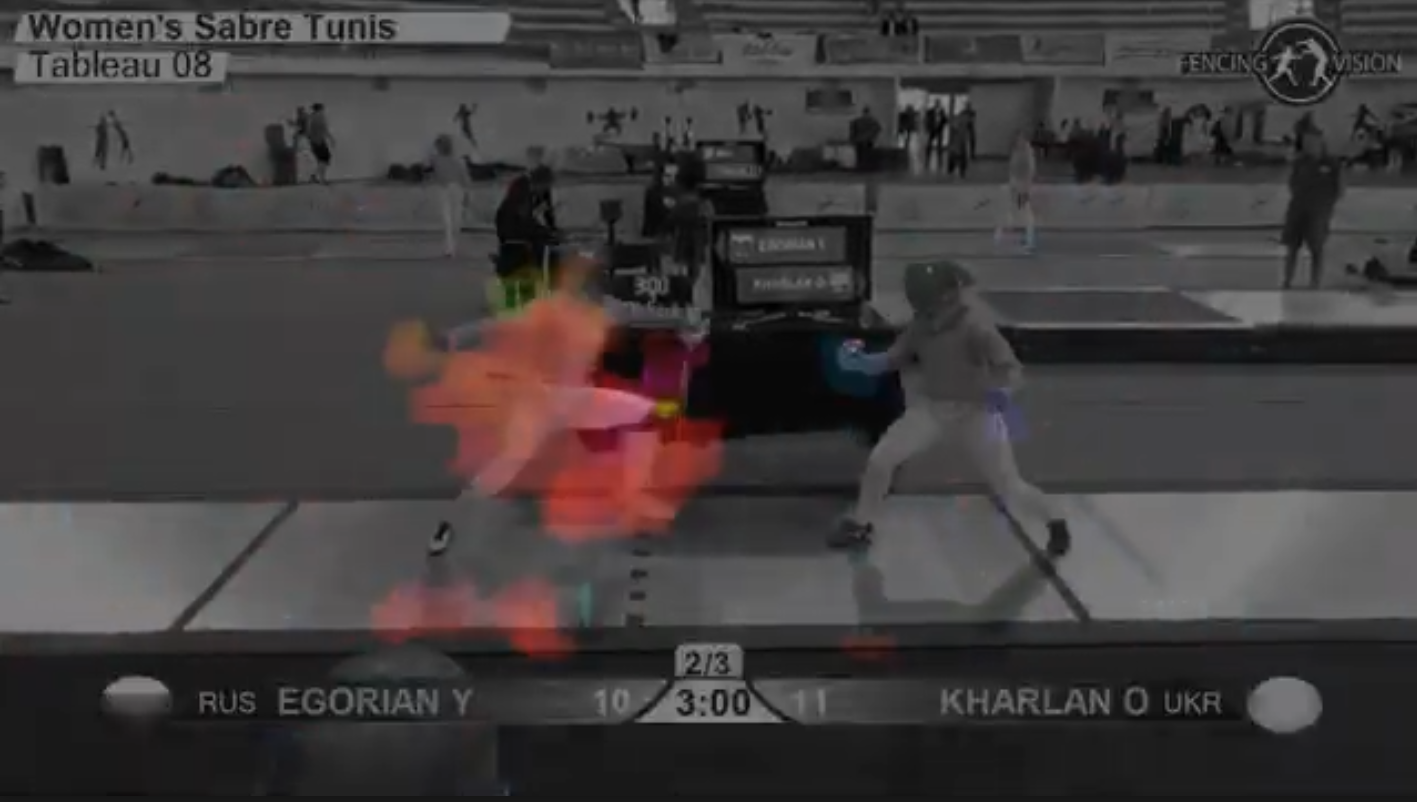
\includegraphics[scale=.21]{overlaid_frame.png}
\caption{A frame overlaid with dense optical flow. We can infer the fencer on the left is moving while the one on the right is more stationary.}
\centering
\end{figure}

\subsection{Convert videos to feature-vector sequences}

This step marks perhaps the biggest departure from Douglas' method.
They used Inception-v3 which was the latest inception model available at their time.
Our decision was to use Inception-v4 which is more efficient.
The aim was to produce a richer feature-vector that encapsulated more of the meaning of each frame.
Frames were individually fed to the CNN and the results were saved in a Pytorch tensor, which was saved to disk in preparation for the next part.
Additionally, some vectors that were too short (<10 frames) were removed.
In total, there were 21,194 clips to feed the RNN.

\subsection{Train an RNN}

The first architecture we attempted to implement was very similar to Douglas'.
It was a single layer LSTM with 500 hidden neurons, followed by two RNN layers with 250 hidden neurons each.
The RNN would take as input the hidden states of the LSTM.
The hope was that the LSTM would encode the long-term information needed for the RNNs to make a decision, while not increasing runtime by using more LSTM layers.
% The second architecture was a similar version of this model, but with increased complexity, using 5 RNN layers with more neurons.
The second model got rid of the RNN layers, instead opting for a more complexity with two LSTMs.
The third and fourth models were variations of this with more LSTM layers.
% The final architecture involved stacking two LSTMs.
This is summarized in table 1.

\begin{table}
\caption{Models used}
\begin{tabular}{l|c}
    \toprule
    model & components \\
    \midrule
    model 1 & LSTM(500) + 2xRNN(250)\\
    model 2 & 2xLSTM(500)\\
    model 3 & 3xLSTM(500)\\
    model 4 & 4xLSTM(500)\\
    \bottomrule
\end{tabular}
\end{table}

\section{Results and analysis}

Over all, the model performed poorer than expected.
The trivial baseline is at 50\%, given that any model can randomly choose between left or right and be correct half the time.
We set a 65\% baseline goal to ensure the model learned a little more than just forward motion.
The best we were able to achieve capped out at 60\% with model 2.
Models 3 and 4, which are very similar but with extra complexity, performed even worse, with model 4 essentially reverting back to a coin-toss.
Though this result isn't what was expected, there are ways to adapt these methods for a better accuracy which require further development.

Training for model 2 used a train-test split of 90-10 given that the dataset was so small to begin with.
A dropout of 0.2 was used during training, and it was run for 10 epochs using the Adam optimizer.

\begin{table}
\caption{Model accuracies}
\begin{tabular}{l|c|c}
    \toprule
    model & components & accuracy \\
    \midrule
    model 1 & LSTM(500) + 2xRNN(250) & 55\%\\
    model 2 & 2xLSTM(500) & 60\%\\
    model 3 & 3xLSTM(500) & 55\%\\
    model 4 & 4xLSTM(500) & 52\%\\
    \bottomrule
\end{tabular}
\end{table}

\begin{figure}
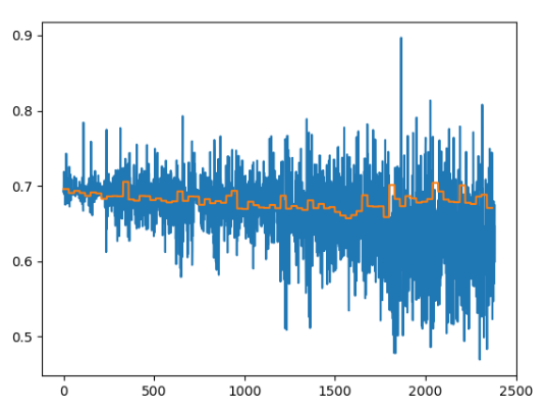
\includegraphics[scale=.6]{trainingloss.png}
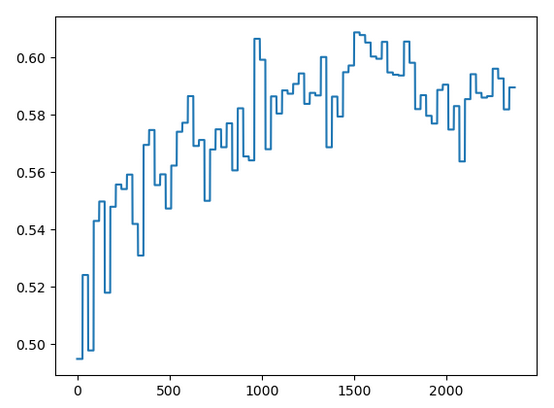
\includegraphics[scale=.6]{trainingacc.png}
\caption{The training loss and accuracy of model 2. The orange line represents validation loss and the blue line represents validation accuracy over \# of batches}
\centering
\end{figure}

\section{Discussion}

Several challenges were encountered over the course of this project.
Since we created the entire pipeline from the data collection stage, there are a plethora of things to tweak to optimize performance.
To combat this, we selected what we thought were optimal parameters and moved on, so as not to waste time early on.
Additionally, a lot of the tasks listed were very computationally intensive.
These operations often required high-performance computing.
Some tasks, namely those that used FFMPEG, couldn't be completed on the HPC cluster used for the rest of the project because of a dependency issue.
So, they had to be completed on a desktop computer with limited RAM and CPU processing power, creating a large time-bottleneck.

To enhance the performance of this model, several steps need to be taken.
Firstly, a more thorough and comprehensive search must be completed of the hyperparameters.
Preferably, all tasks would be ported to an HPC environment for faster prototyping and development.
Another consideration is the dataset used.
One of the biggest things holding this model back is the input dataset size.
We used videos from a single tournament to ensure the HUD remains the same across videos.
However, it's possible that there are other tournaments which use the same HUD, so these could add to the number of videos available to train on.
Other suggestions include more intelligent frame cropping or masking, to avoid feeding useless background data to the model.
Finally, we intend to explore different models for the feature-vector extraction step, such as ResNet models.

A very interesting idea we explored very early on was using pose estimation to detect keypoints on the fencers bodies.
This way, instead of feeding each frame through a feature-vector extractor, we could instead extract pose data.
This would---in theory---be less noisy than an image since it wouldn't contain irrelevant pixel data.
However, we couldn't find a suitable pose estimation model for this task.
We looked at popular options like \textit{OpenPose} and \textit{MediaPipe}.
The former seemed to be abandonware with no working build instructions.
The latter struggled with keeping focus on the same fencer over time.
This created choppy and noisy detections, which rarely related to the actual occurring action.
Perhaps, in the future, the state of the art will advance and this option will be more viable.

\section{What we learned}

This project included a lot of data processing steps.
We implemented many solutions to common problems for training neural networks on video data, including creating a new algorithm to label score changes.
We also explored dense optical flow methods and techniques to help CNNs retain motion/time-data.
Pose estimation was also a topic of interest, though we weren't able to find anything fruitful.
Finally, we used a high performance computing cluster, the use of which helped teach many HPC practices and considerations, including job scheduling.

\end{document}
